\section{Running Example: the Heterogeneous Model of a Coffee Machine}
\label{sec:runningexample}
\begin{itemize}
	\item In this section, we model a coffee machine that is composed by two subsystems: one that controls the insertion of a coin and other that does the coffee. In the following, we model each subsystem by using a dedicated language.
	
	\item The behavior of the subsystem that controls the locking and unlocking of the coffee machine is described as follows: when a coin is inserted, the event selectCoffee is triggered and the machine becomes unlocked. Then, when the releseCoffee event happens, the machine becomes locked again. 
	\item To model this subsystem, we use a state-based language named TFSM. This is a state machine language augmented with timed transitions (see Figure~\ref{fig:tfsmmm}). The metamodel describes the abstract syntax of the TFSM language (see Figure~\ref{fig:tfsmmm}). A \emph{System} is composed of \emph{TFSMs}, global \emph{FSMEvents} and global \emph{FSMClocks}. Each \emph{TFSM} is composed of \emph{States}. Each state can be the source of outgoing guarded \emph{Transitions}. A guard can be specified either by the reception of an \emph{FSMEvent} (\emph{EventGuard}) or by a duration relative to the entry time in the source state of the transition (\emph{TemporalGuard}). When fired, transitions generate a set of simultaneous \emph{FSMEvent} occurrences.
	
	\item The TFSM language defines the following \dse: \emph{entering} and \emph{leaving} a state, \emph{firing} a transition, the occurrences (\emph{occurs}) of a FSMEvent and the \emph{ticks} of a FSMClock (see at the top of Figure~\ref{fig:tfsmmm}). These \dse are part of the language behavioral interface of TFSM. \dse are defined by using a specific language named \ecl (standing for Event Constraint Language~\cite{ECL}) which is an extension of OCL~\cite{omgocl2} with events. \ecl takes benefits from the OCL query language and its possibility to augment an abstract syntax with additional attributes (without any side effects). Consequently, by using \ecl, it is possible to augment \as metaclasses and add \dse. A partial \ecl specification of TFSM is shown in Listing~\ref{fig:tfsmmmecl} where the \dse \textit{entering} and \textit{leaving} are defined in the context of State (Listing~\ref{fig:tfsmmmecl}: line 6) while \textit{occurs} is defined in the context of FSMEvent (Listing~\ref{fig:tfsmmmecl}: line 4). When a metaclass is instantiated, the corresponding \dse are instantiated; \eg for each instance of the metaclass \emph{State}, \dse \textit{entering} is instantiated. 
	
	\item Each instance of \dse is a \mse. 
	
	\item We use this language to build the TFSM named \emph{CoffeeCoin} (see Figure~\ref{fig:tfsmmm}). The model is composed by two States (\emph{Locked} and \emph{Unlocked}). So that there are two \mse of \textit{entering}: \textit{Locked} and \textit{Unlocked}. All \mse are part of the model behavioral interface. 
	
	\item The second subsystem is the sequential procedure of make coffee: first the coffee is selected, second it is built, and then it is released. To model this procedure, we use an action-based language named Activity Language. 
	
	\item Figure~\ref{fig:activitymm} shows the partial metamodel of Activity (see~\cite{ttc15bib}). The root element is an \emph{Activity} that is composed by \emph{ActivityNodes} and \emph{ActivityEdges}. Each ActivityNode can be the source of the outgoing ActivityEdges. The language behavioral interface of the Activity is partially shown in  Listing~\ref{fig:eclfuml}. For each \emph{Activity} two \dse are defined: \emph{startActivity} and \emph{finishActivity}, to identify respectively the starting and finishing instants of the activity. One \dse is defined for each \emph{Action}: \emph{executeIt}, to identify the execution of an Action.

	\item We use this language to build the activity named \emph{CoffeeAlgorithm} (see Figure~\ref{fig:activitymm}). The model behavioral interface is made of three \mse of \emph{executeIt}: \emph{selectCoffee}, \emph{makeCoffee} and \emph{releaseCoffee}. Also, it contains one \mse of \emph{startActivity} and \emph{finishActivity} named respectively \emph{CoffeeAlgorithm:startActivity} and \emph{CoffeeAlgorithm:finishActivity}.
	
	\item These models interact: when TFSM becomes unlocked and the FSMEvent selectCoffee is triggered the Action selectCoffee is executed. Then, when the Action releaseCoffee is executed, the FSMEvent releaseCoffee is triggered and the TFSM becomes locked again.
	
	\item The coordination between these models can be specified by defining constraints between the \mse in the interface. For instance, we need to specify how the \mse \emph{executeIt:selectCoffee} and \emph{occurs:selectCoffee} are synchronized. 

	\item To illustrate the use of \bcool, we propose a simple running example \ie, building an operator that coordinates FSMEvents from TFSM and Actions from Activity by relying on their names. We informally define it as follows: When coordinating a TFSM and an Activity, all pairs of FSMEvents and Actions that have the same name must be synchronized using a \emph{rendez-vous}. The operator is defined for any pair of TFSM and Activity. When applied it concerns two specific state machines, at the instance (model) level. In the following section, we present the syntax and the semantic of \bcool.
	
\end{itemize}



\begin{figure}
	\begin{center}
		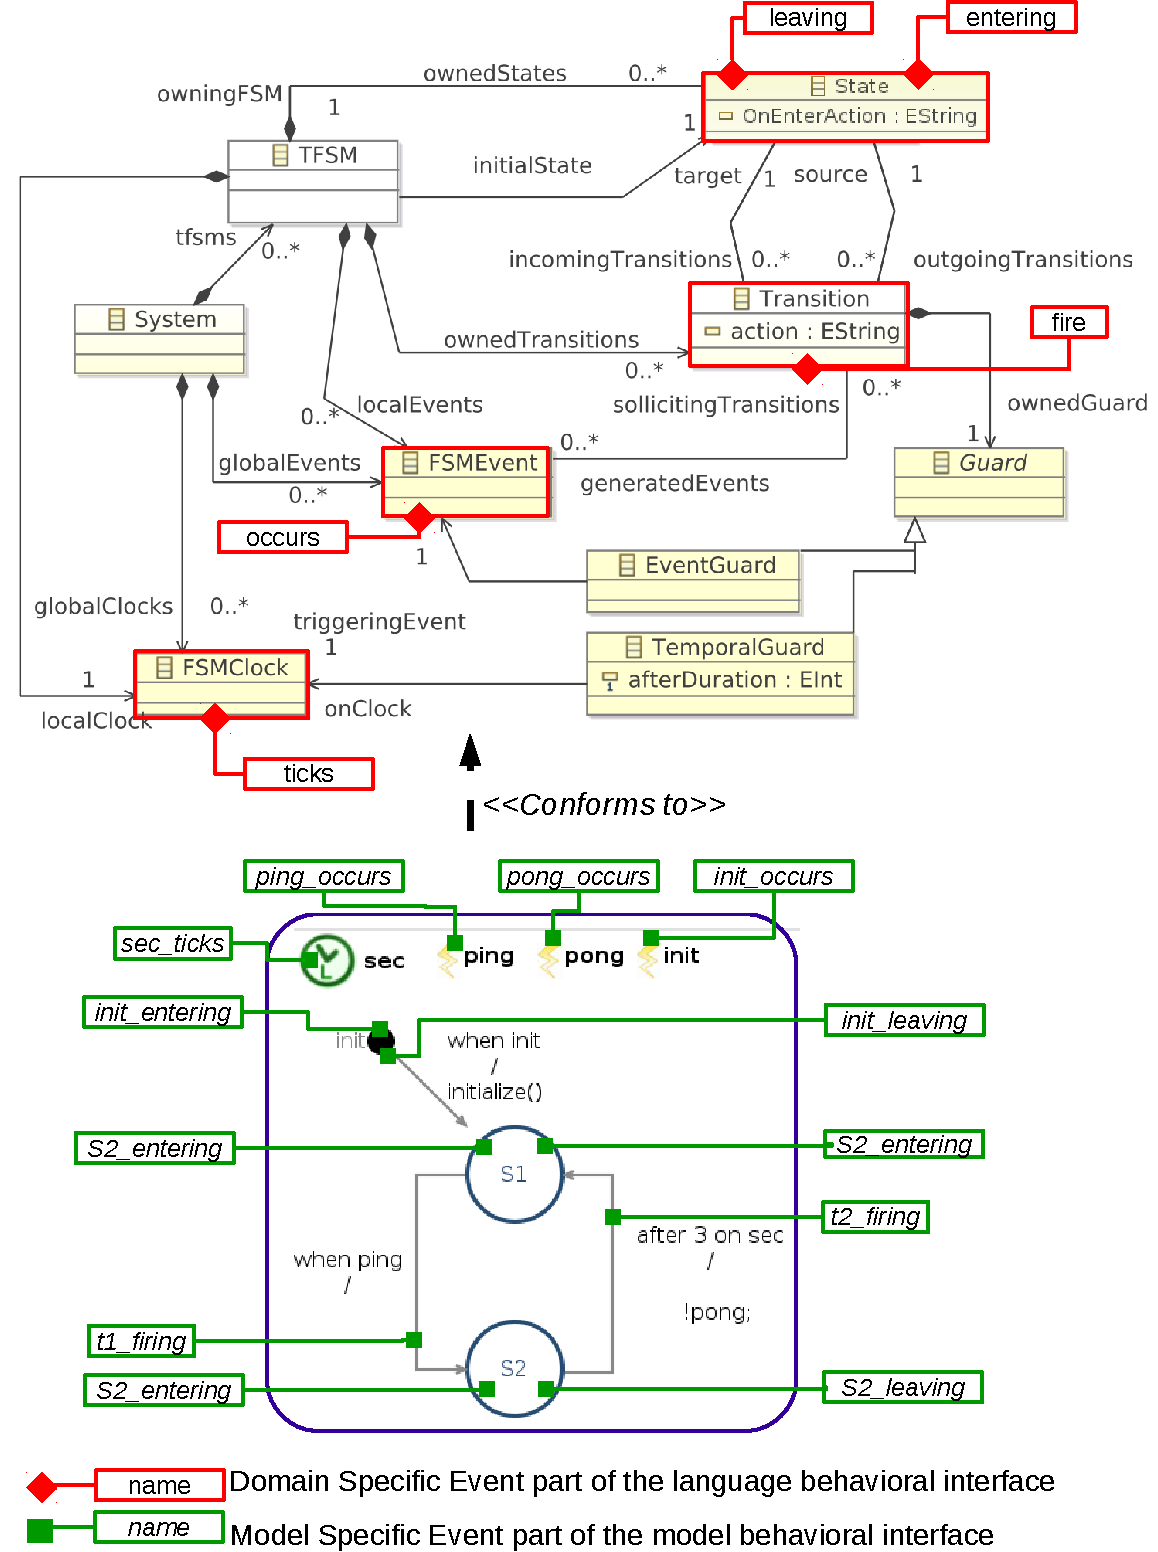
\includegraphics[width=1\textwidth]{bcool/figs/tfsmlang}
		\caption{(At the top) The TFSM metamodel with its language behavioral interface. (At the bottom) a TFSM model with its model behavioral interface}
		\label{fig:tfsmmm}
	\end{center}
\end{figure}

\begin{figure}
	\center
	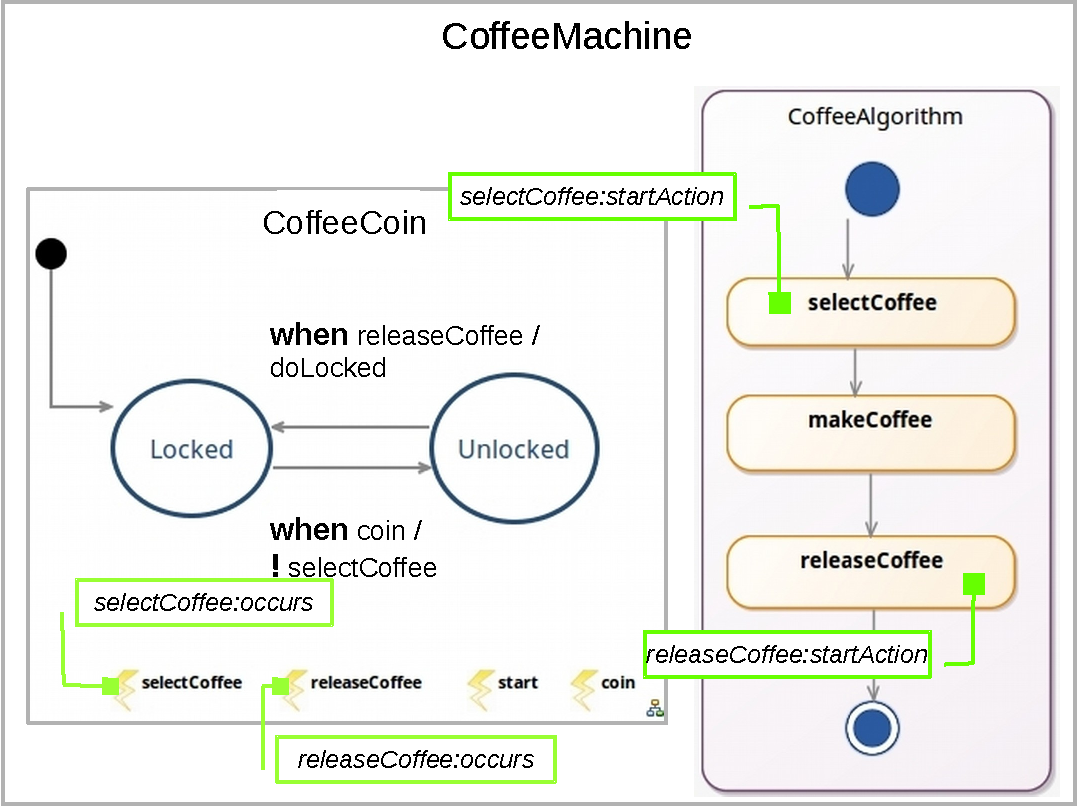
\includegraphics[width=.5\columnwidth]{bcool/figs/models.pdf}
	\caption{Heterogeneous Model of a Coffee Machine}
	\label{fig:runningexample}
\end{figure}

\begin{lstlisting}[language=ecl,
caption={Partial \ecl specification of TFSM},
label={fig:tfsmmmecl}, 
basicstyle=\scriptsize\ttfamily, backgroundcolor=\color{LGrey}, numbers=left, xleftmargin=3pt]
package tfsm
context FSMClock
def: ticks : Event = self
context FSMEvent
def: occurs : Event = self
context State
def : entering : Event = self
def : leaving : Event = self
\end{lstlisting}


\begin{figure}
	\begin{center}
		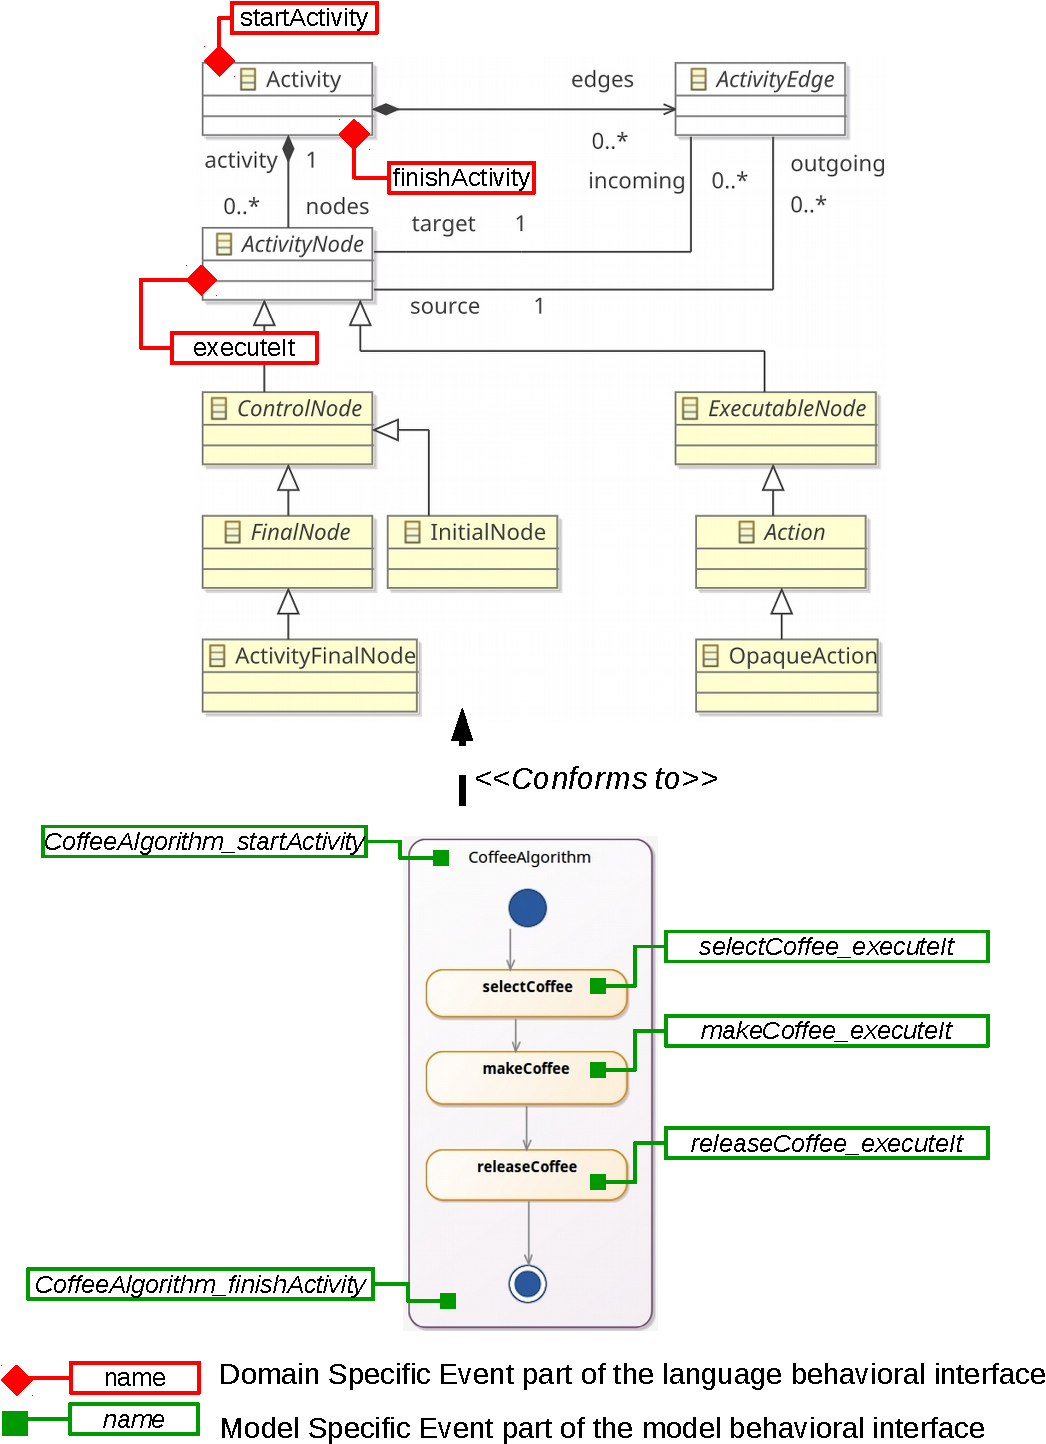
\includegraphics[width=1\textwidth]{bcool/figs/activitylang}
		\caption{(At the top) The Activity metamodel with its language behavioral interface. (At the bottom) an Activity model with its model behavioral interface}
		\label{fig:activitymm}
	\end{center}
\end{figure}


\begin{lstlisting}[language=ecl,
caption={Partial \ecl specification of Activity Diagram},
label={fig:eclfuml}, 
basicstyle=\scriptsize\ttfamily, backgroundcolor=\color{LGrey}, numbers=left, xleftmargin=3pt, belowskip=-0.4em]
package uml
context Activity
def: startActivity : Event = self
def: finishActivity: Event = self
context Action
def : startAction : Event = self
def : finishAction : Event = self
\end{lstlisting}
